\uuid{6dR4}
\titre{ Associer une fonction à ses courbes de niveau }

\niveau{}
\module{ Fonctions de plusieurs variables }
\chapitre{Courbe de niveau}
\sousChapitre{Représentation graphique}
\theme{}
\auteur{Quentin Liard}
\datecreate{ 2026-03-18}
\organisation{}
\difficulte{}

\contenu{

\texte{ 
On considère les quatre fonctions suivantes :

\[
f_1(x,y)=xy,
\qquad
f_2(x,y)=\frac{y}{x},
\qquad
f_3(x,y)=x^2+y^2,
\qquad
f_4(x,y)=x^2-y.
\]

On donne ci-dessous quatre représentations de familles de courbes de niveau, notées (A), (B), (C) et (D).

Associer à chaque fonction la bonne famille de courbes de niveau. Justifier soigneusement chaque réponse.

\medskip

\begin{center}

\begin{minipage}{0.48\textwidth}
\centering
\textbf{(A)}

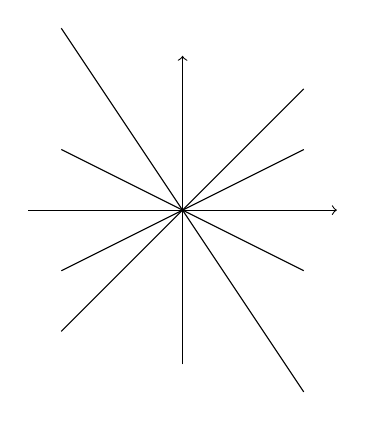
\begin{tikzpicture}[scale=0.7]
\draw[->] (-2.8,0)--(2.8,0);
\draw[->] (0,-2.8)--(0,2.8);
\draw[domain=-2.2:2.2,samples=100] plot (\x,{0.5*\x});
\draw[domain=-2.2:2.2,samples=100] plot (\x,{1*\x});
\draw[domain=-2.2:2.2,samples=100] plot (\x,{-0.5*\x});
\draw[domain=-2.2:2.2,samples=100] plot (\x,{-1.5*\x});
\end{tikzpicture}
\end{minipage}
\hfill
\begin{minipage}{0.48\textwidth}
\centering
\textbf{(B)}

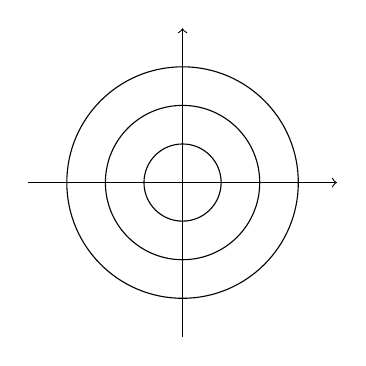
\begin{tikzpicture}[scale=0.7]
\draw[->] (-2.8,0)--(2.8,0);
\draw[->] (0,-2.8)--(0,2.8);
\draw (0,0) circle (0.7);
\draw (0,0) circle (1.4);
\draw (0,0) circle (2.1);
\end{tikzpicture}
\end{minipage}

\vspace{0.8cm}

\begin{minipage}{0.48\textwidth}
\centering
\textbf{(C)}

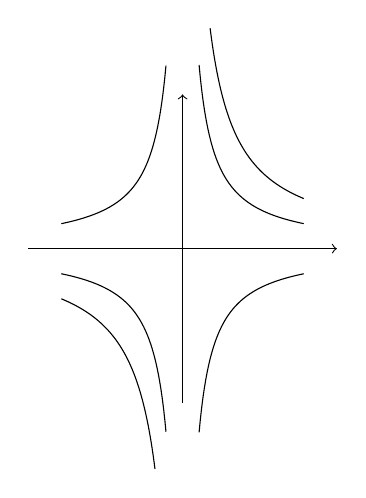
\begin{tikzpicture}[scale=0.7]
\draw[->] (-2.8,0)--(2.8,0);
\draw[->] (0,-2.8)--(0,2.8);
\draw[domain=-2.2:-0.3,samples=100] plot (\x,{1/\x});
\draw[domain=0.3:2.2,samples=100] plot (\x,{1/\x});
\draw[domain=-2.2:-0.3,samples=100] plot (\x,{-1/\x});
\draw[domain=0.3:2.2,samples=100] plot (\x,{-1/\x});
\draw[domain=-2.2:-0.5,samples=100] plot (\x,{2/\x});
\draw[domain=0.5:2.2,samples=100] plot (\x,{2/\x});
\end{tikzpicture}
\end{minipage}
\hfill
\begin{minipage}{0.48\textwidth}
\centering
\textbf{(D)}

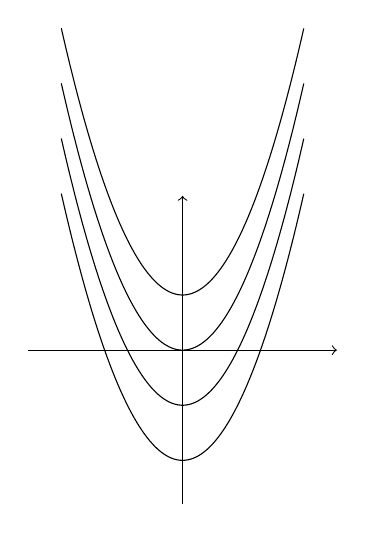
\begin{tikzpicture}[scale=0.7]
\draw[->] (-2.8,0)--(2.8,0);
\draw[->] (0,-2.8)--(0,2.8);
\draw[domain=-2.2:2.2,samples=100] plot (\x,{\x*\x-2});
\draw[domain=-2.2:2.2,samples=100] plot (\x,{\x*\x-1});
\draw[domain=-2.2:2.2,samples=100] plot (\x,{\x*\x});
\draw[domain=-2.2:2.2,samples=100] plot (\x,{\x*\x+1});
\end{tikzpicture}
\end{minipage}

\end{center}
}


}